\section{Topologías ferroviarias}

    Las redes ferroviarias presentan dos piezas fundamentales en su infraestructura: su topología (la traza ferroviaria) y los elementos ferroviarios que la componen. La topología es el entramado de vías férreas conectadas de forma arbitraria, cuyo diseño busca cumplir una función particular, interconectando diversos elementos ferroviarios. Estos elementos pueden ser para determinar la ubicación del tren, para delimitar la circulación de vehículos en cruces ferroviarios, permitir el ascenso y descenso de pasajeros, o para modificar dinámicamente los caminos por los que los trenes circulan, entre otras funciones.

    Cualquiera sea el elemento involucrado, altera las funciones de la red y su inminente proximidad debe informarse cuanto antes al conductor del tren. Este podrá decidir, de estar permitido, modificar o no su accionar antes de alcanzar dicho elemento. Es tarea del señalamiento ferroviario alertar a los conductores ferroviarios de cualquier elemento que pueda representar un peligro, evitando así colisiones con otras formaciones o descarrilamientos en zonas críticas. El señalamiento ferroviario incluye un elemento fundamental: los semáforos.

    Los semáforos (de ahora en mas denominados "señales"), constituyen el medio de comunicación primario entre los conductores y su entorno, informándoles de la habilitación o denegación de uso de las vías posteriores mediante su color, denominado aspecto. Cada señal puede presentar un único aspecto por vez de un conjunto posible que varía según el país o la región. Los aspectos utilizados en Argentina son el verde (permitido avanzar), amarillo (atención) y rojo (detenerse). Algunas señales pueden no tener el aspecto verde (señales de maniobras de dos aspectos) o incorporar un aspecto extra entre el rojo y el amarillo (señales de cuatro aspectos que incluyen el doble amarillo).
    
    Dos señales consecutivas con la misma dirección y sentido constituyen una ruta ferroviaria. Los operarios ferroviarios solicitan al sistema de enclavamientos las rutas que necesitan en base a la logística deseada. El sistema de enclavamientos habilitará o denegará las rutas solicitadas en función del estado de los elementos ferroviarios cercanos y de las demás rutas activas. Esta función es vital para el sistema ferroviario y su fin último es permitir la circulación de trenes de la forma mas segura o, de no ser posible, no permitir circulación alguna.

    \subsection{Derivación ferroviaria}

Cuando es necesario interconectar dos puntos separados por una distancia de decenas o cientos de kilómetros donde hay poco tráfico ferroviario, resulta económicamente poco conveniente construir vías en ambos sentidos. No obstante, construir una sola vía bidireccional presenta inconvenientes logísticos notorios: una formación que circule entre los puntos A y B excluye a cualquier formación que quiera circular de B a A sin colisionar. %No sería posible utilizar la infraestructura en el sentido opuesto mientras se encuentre ocupada.

La solución mas utilizada emplea islas de enclavamiento a modo de bypass cada cierta cantidad de kilómetros, como se ilustra en la Figura \ref{fig:bypass_1}. Estas islas permiten que las formaciones puedan cruzarse sin riesgo de colisión. La primer formación en llegar a la isla de enclavamientos accede al bypass por la vía superior y espera a que la formación en sentido contrario circule por la vía inferior. Una vez despejado el camino que resta por recorrer, la formación reingresa a la vía principal y retoma su marcha.

    \begin{figure}[h]
        \centering
        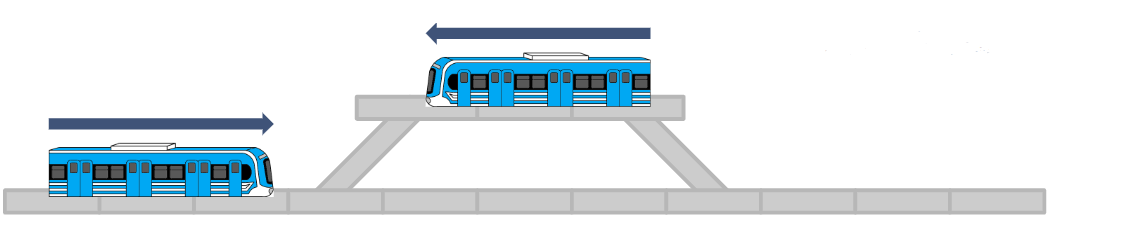
\includegraphics[width=1\textwidth]{Figuras/bypass}
        \centering\caption{Topología de derivación ferroviaria.}
        \label{fig:bypass_1}
    \end{figure}
    
Las topologías de derivación ferroviaria se utilizan principalmente para transportar materias primas entre locaciones rurales a grandes distancias de los puestos. Es deseable tanto una logística óptima, para transportar mas bienes y mas rápido, cómo un sistema seguro que garantice que los bienes lleguen a destino.
    \subsection{Simple}

En entornos urbanos donde las estaciones ferroviarias se encuentran separadas entre sí por unos pocos kilómetros es necesaria una interconectividad mayor. El sistema ferroviario debe satisfacer la demanda de una población mayor y a la vez coexistir con un trazado vehicular mucho mas denso que cruza al trazado ferroviario en varios puntos. En este contexto, una topología simple como la presentada en la Figura \ref{fig:simple_1} es una solución óptima al problema planteado.

    \begin{figure}[h]
        \centering
        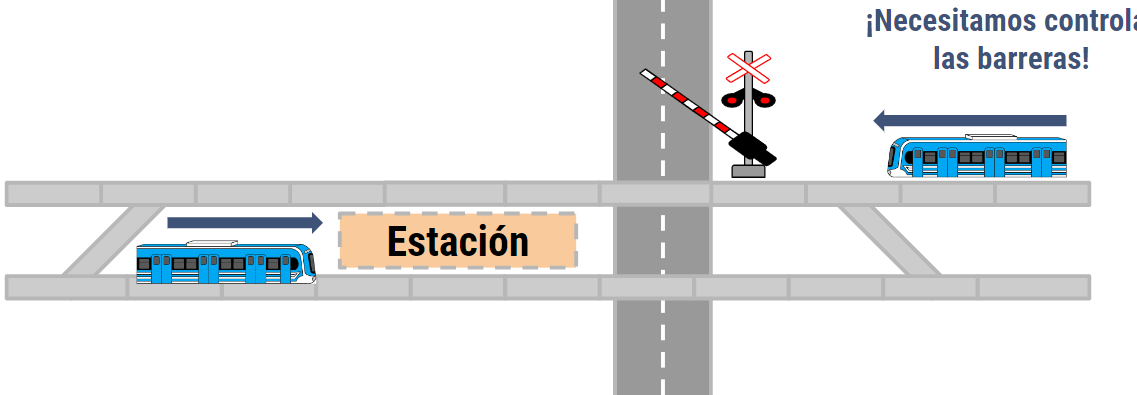
\includegraphics[width=1\textwidth]{Figuras/simple}
        \centering\caption{Topología simple.}
        \label{fig:simple_1}
    \end{figure}

El cruce entre el trazado ferroviario y el trazado vehicular se denomina paso a nivel. El sistema de enclavamientos deberá garantizar que el paso a nivel se encuentre despejado de vehículos y peatones antes de permitir la circulación de trenes sobre el mismo. Esto se logra mediante el uso de una barrera ferroviaria, un mecanismo que mantiene la barrera en alto mientras no se detecten formaciones en las proximidades del paso a nivel.

Las topologías simples suelen contar con dos vías unidireccionales en sentido ascendente y descendente. 
Las vías ascendentes son aquellas por las que las formaciones circulan en la dirección del kilometraje creciente. Mientras que las vías descendentes son aquellas por las que circulan en la dirección del kilometraje decreciente [REF]. El kilómetro cero es la estación principal de la línea ferroviaria, como por ejemplo: Plaza Constitución (Línea Roca), Once de Septiembre (Línea Sarmiento) o Retiro (Línea Mitre y Linea San Martín). Las formaciones pueden cambiar de vía ascendente a descendente, o viceversa, utilizando un cambio ferroviario.
    \subsection{Hub}

A medida que mas líneas ferroviarias coexisten en la misma red se vuelve inevitable que varias líneas compartan la misma estación utilizando diferentes plataformas en paralelo. Con una logística mas flexible, las diferentes líneas incluso pueden utilizar de forma alternada las mismas plataformas y, por lo tanto, las mismas vías principales. Además, es necesario contar con mecanismos para retirar trenes de la red para su mantenimiento y volver a inyectarlos a la red cuando la demanda aumente. Esto se logra por medio de talleres ferroviarios en las inmediaciones de las estaciones que actúan como un hub ferroviario. La topología de hub ferroviario se ilustra en la Figura \ref{fig:hub_1}.

    \begin{figure}[h]
        \centering
        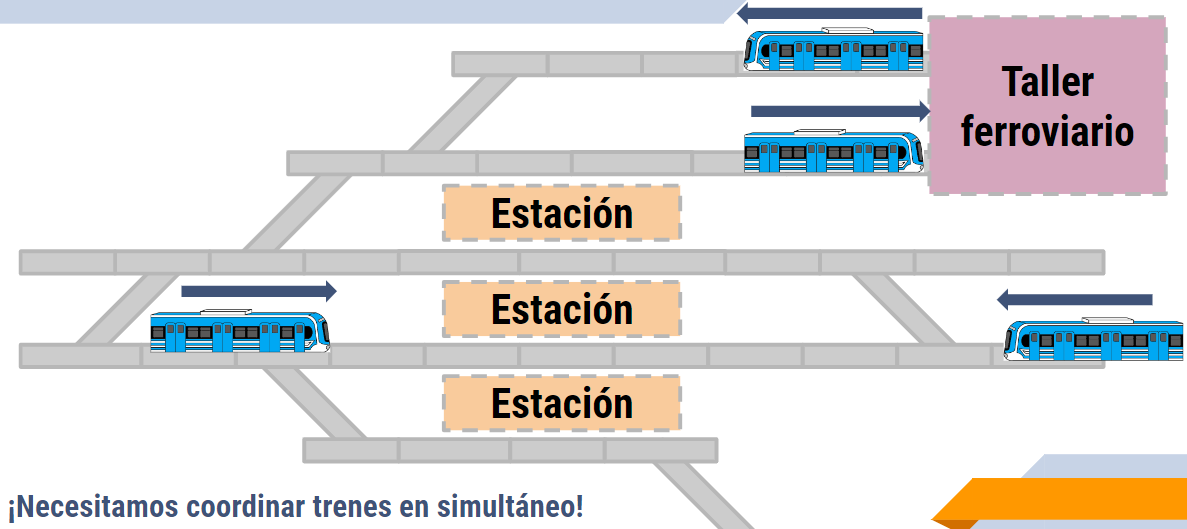
\includegraphics[width=1\textwidth]{Figuras/hub}
        \centering\caption{Topología hub.}
        \label{fig:hub_1}
    \end{figure}
    
Las tareas del sistema de enclavamientos van aumentando en complejidad a medida que se suman nuevos actores. Debe coordinar diversas formaciones de distintas líneas, accediendo a diferentes plataformas, cumpliendo diferentes horarios de arribo y partida. A su vez, debe asegurarse de que las formaciones circulen con seguridad pero sin descuidar la puntualidad. Adicionalmente, debido a que la demanda varía a lo largo del día, deberá tener flexibilidad para inyectar nuevas formaciones a la red o remover las que presenten desperfectos técnicos. Todas estas acciones deben realizarse en simultáneo y en un entorno de alto dinamismo.
    \subsection{Estación Terminal}

Las estaciones terminales presentan una gran cantidad de vías principales y plataformas en paralelo, en las cuales confluyen una o varias líneas ferroviarias. A diferencia de estaciones de tipo hub que pueden presentar finales de vía relativos, las estaciones terminales poseen finales de vía absolutos. Es decir, las formaciones que circulan por la vía descendente deberán detener su marcha completamente antes de llegar al fía de vía, para luego retomar su marcha en sentido contrario, por la vía ascendente. Esta operación puede realizarse de manera inmediata en formaciones con locomotras eléctricas en ambos extremos del tren o con locomotoras diesel luego de varias maniobras que requieren el uso de diversos cambios de vías. En la Figura \ref{fig:terminal_1} se ilustra un ejemplo de una estación terminal.

    \begin{figure}[h]
        \centering
        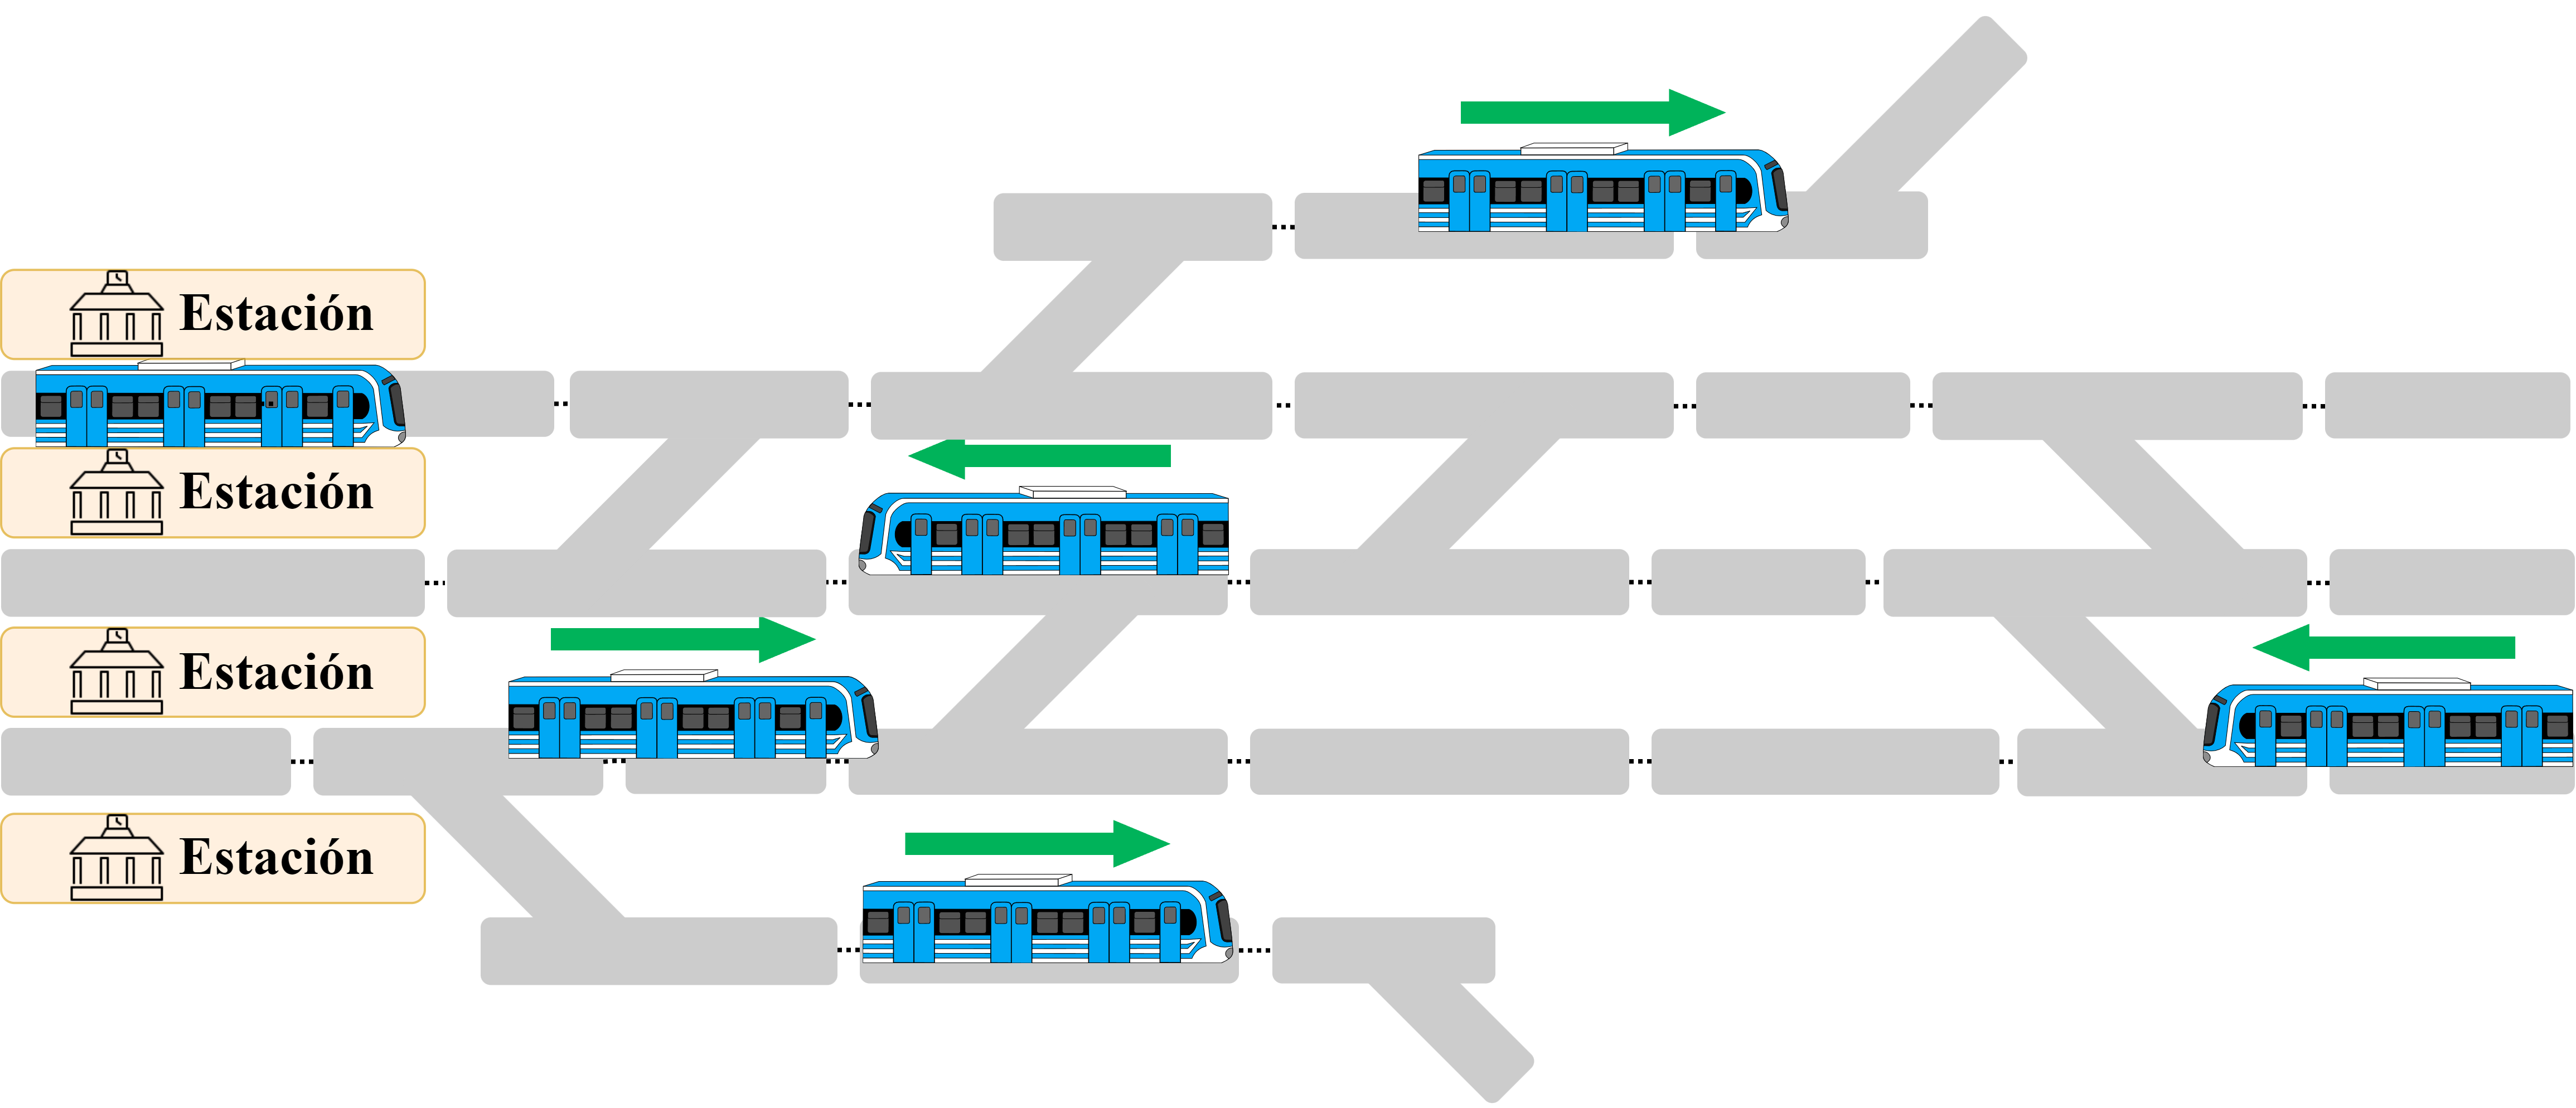
\includegraphics[width=1\textwidth]{Figuras/terminal}
        \centering\caption{Topología terminal.}
        \label{fig:terminal_1}
    \end{figure}

En las estaciones terminales suelen confluir la información en tiempo real de la terminal y las estaciones mas próximas de la línea, o incluso la información en tiempo real de la totalidad de la línea. Esta característica, además de ser la estación de mayor tamaño de la línea, les otorga una jerarquía tal que suelen concentrar parcial o totalmente el control del señalamiento de la red. Las decisiones tomadas en una estación terminal tienen un gran impacto en el sistema de transporte de toda la línea, directa o indirectamente. Estas operaciones deben considerar cientos o miles de estados en simultáneo, por lo que ejecutarlas de forma manual es muy complejo o incluso imposible. Un sistema de enclavamientos moderno, robusto, que pueda garantizar una altísima disponibilidad, mantenibilidad y seguridad es indispensable para llevar a cabo estas tareas.
    \subsection{Complejas}

\lipsum[1]
\includegraphics{example-image}
\lipsum[1]